%DO NOT MESS AROUND WITH THE CODE ON THIS PAGE UNLESS YOU %REALLY KNOW WHAT YOU ARE DOING

\chapter{Exercises with Matlab}


\section{ Sample covariance function } \label{ Sample covariance function } 
\lstset{language=Matlab,%
    %basicstyle=\color{red},
    basicstyle=\scriptsize,
    breaklines=true,%
    morekeywords={matlab2tikz},
    keywordstyle=\color{blue},%
    morekeywords=[2]{1}, keywordstyle=[2]{\color{black}},
    identifierstyle=\color{black},%
    stringstyle=\color{mylilas},
    commentstyle=\color{mygreen},%
    showstringspaces=false,%without this there will be a symbol in the places where there is a space
    emph=[1]{for,end,break},emphstyle=[1]\color{red}, %some words to emphasise
    %emph=[2]{word1,word2}, emphstyle=[2]{style},    
}
\noindent \textbf{Task:} Write a function \texttt{covfct} for determining the sample and the modified sample covariance function. To calculate both sample covariance functions take the first 200 random numbers from \texttt{dat1\_1}. Display the results and explain the differences between the functions. What indicates that a sequence of random numbers can be interpreted as a realisation of discrete white noise?
(Note: In MATLAB exists a similar function \texttt{xcov}. Ascertain the correctness of your function \texttt{covfct} by comparing the results of the experiments with \texttt{covfct} and \texttt{xcov}.)

\noindent \textbf{Solution:}
\noindent First, we save the first 200 random numbers from \texttt{dat1\_1} in a variable \texttt{X}. We then wrote a function \texttt{covfct} to determine the sample and modified sample covariance function. We also used a similar function, \texttt{xcov} built by MATLAB in-order to compare our results with the results from this function. A sequence of random numbers can be interpreted as a realization of discrete white noise if the mean is zero and there is no correlation between two different numbers as the variance of a discrete white noise is,
$$ C_{xx}(t) = {\sigma_Z}^2 \delta_\tau    $$
\noindent \textbf{MATLAB code:}
\lstinputlisting{assignment4_1.m}

\noindent \textbf{Output:}
\noindent Figure 2.1 (a) shows the output by the \texttt{covfct} which Figure 2.1 (b) shows the simulated output of the matlab function \texttt{xcov} with biased argument. This means that the mean value is known.
\begin{figure}[H]
    \centering
   \subfloat[Sample Covariance]{ {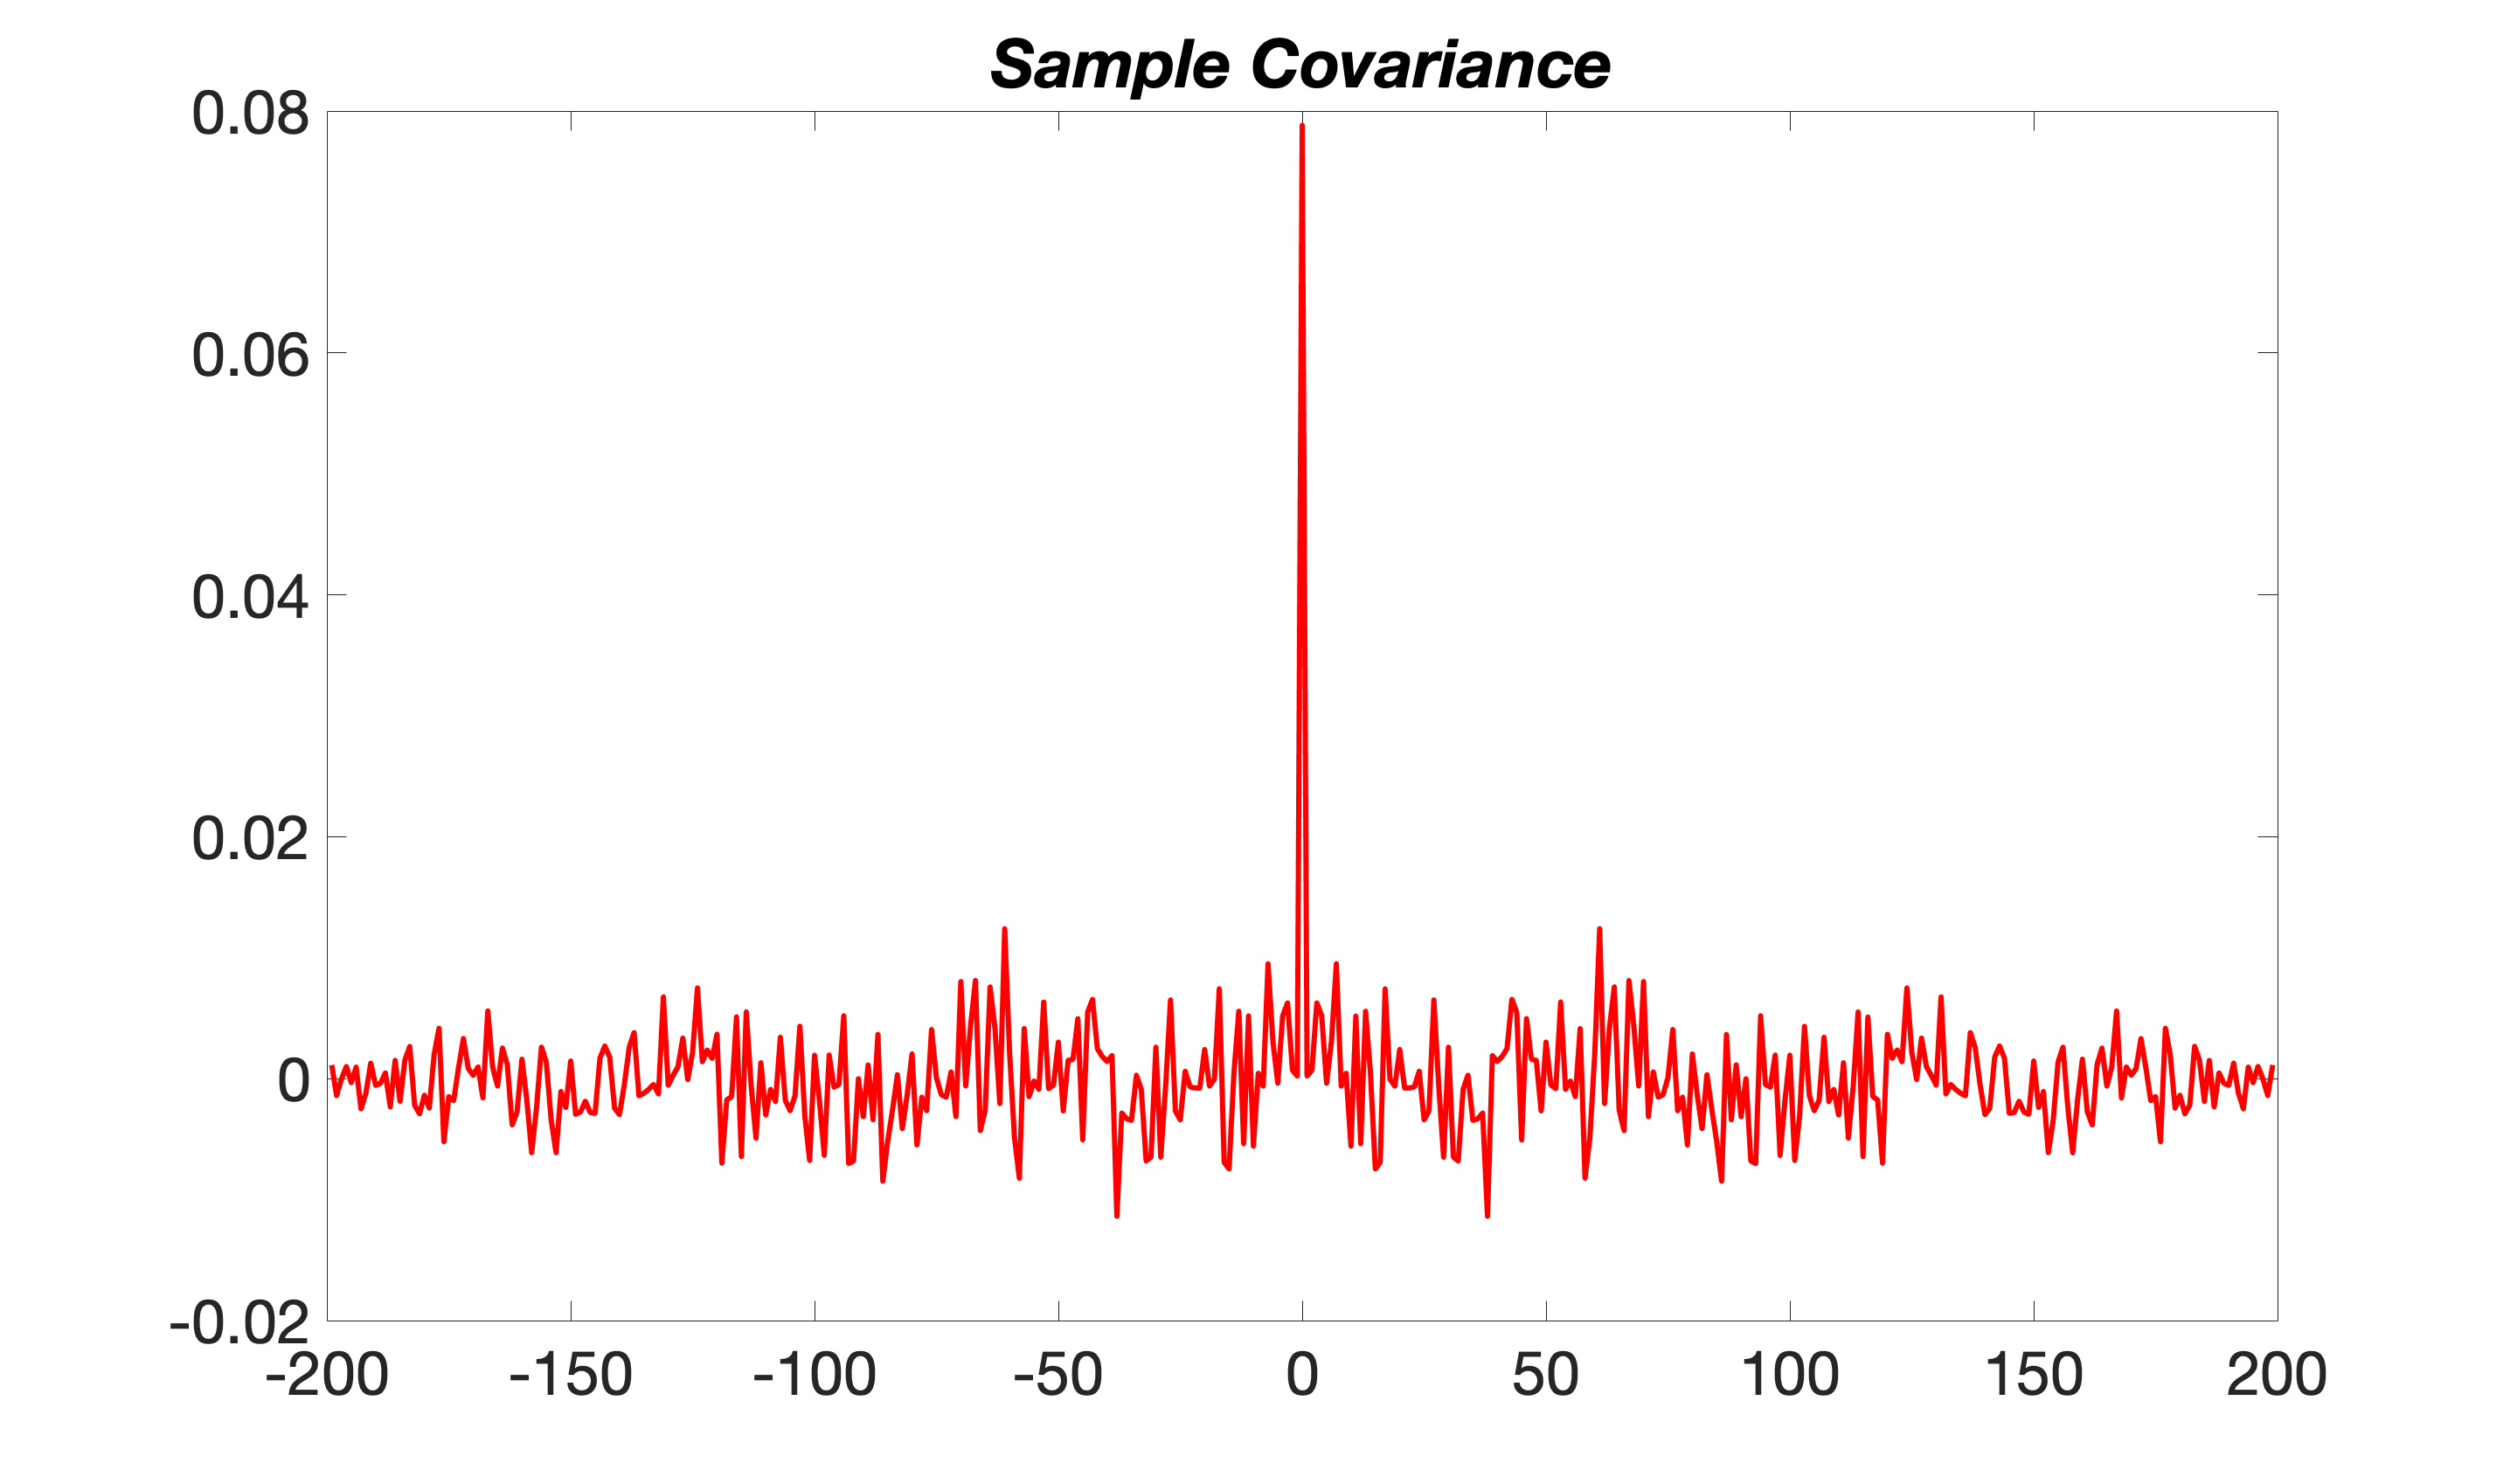
\includegraphics[width=8cm]{ass1_1.png}} }
    \qquad
    \subfloat[Biased Covariance]{ {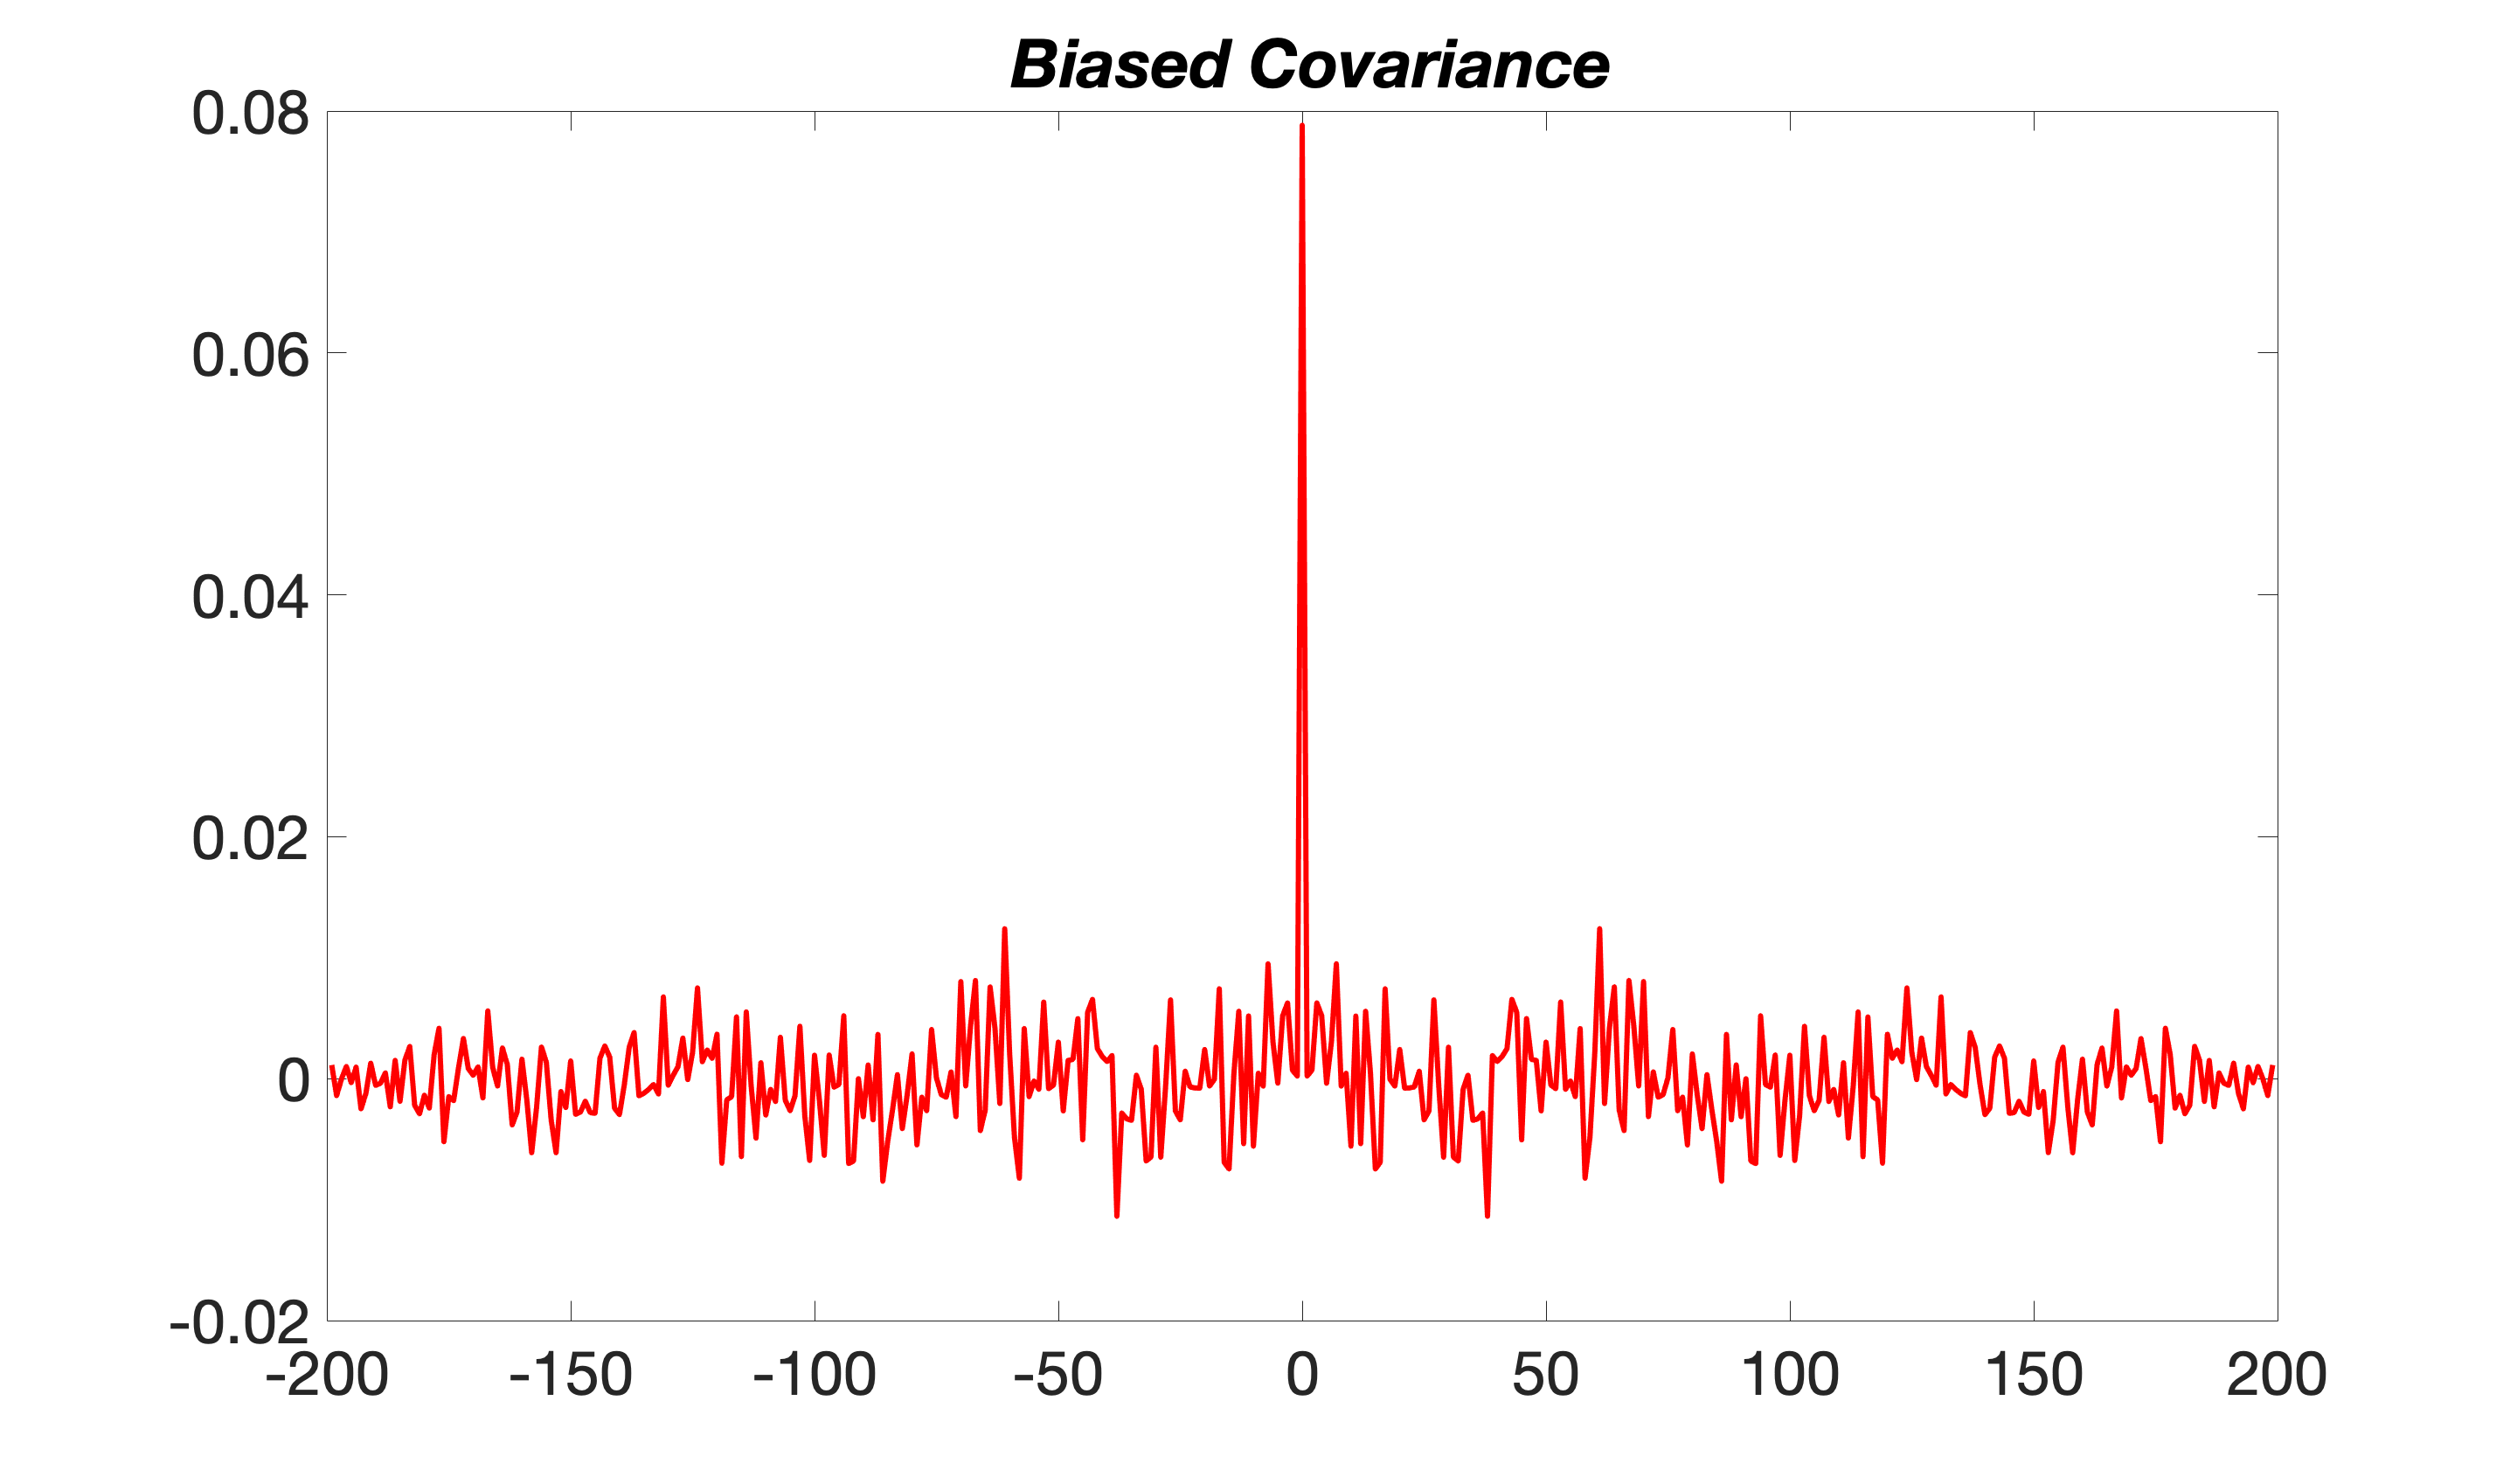
\includegraphics[width=8cm]{ass1_3.png} }}
   % \label{Covariances found using functions \texttt{covfct} and \texttt{xcov}}
    \caption{Covariances found using functions \texttt{covfct}(Sample) and \texttt{xcov}(Biased)}
\end{figure}
\noindent Similarly Figure 2.2 (a) shows the output by the \texttt{covfct} which Figure 2.1 (b) shows the simulated output of the matlab function \texttt{xcov} with unbiased argument. This means that the mean value is known. The point that there is a peak at the center of this sample covariance function means it shall be white noise in wide
sense stationary, the \texttt{xcov} also shows almost no cross-correlation and peak at the center with symmetry at both sides.
\begin{figure}[H]
    \centering
   \subfloat[Modified Sample Covariance]{ {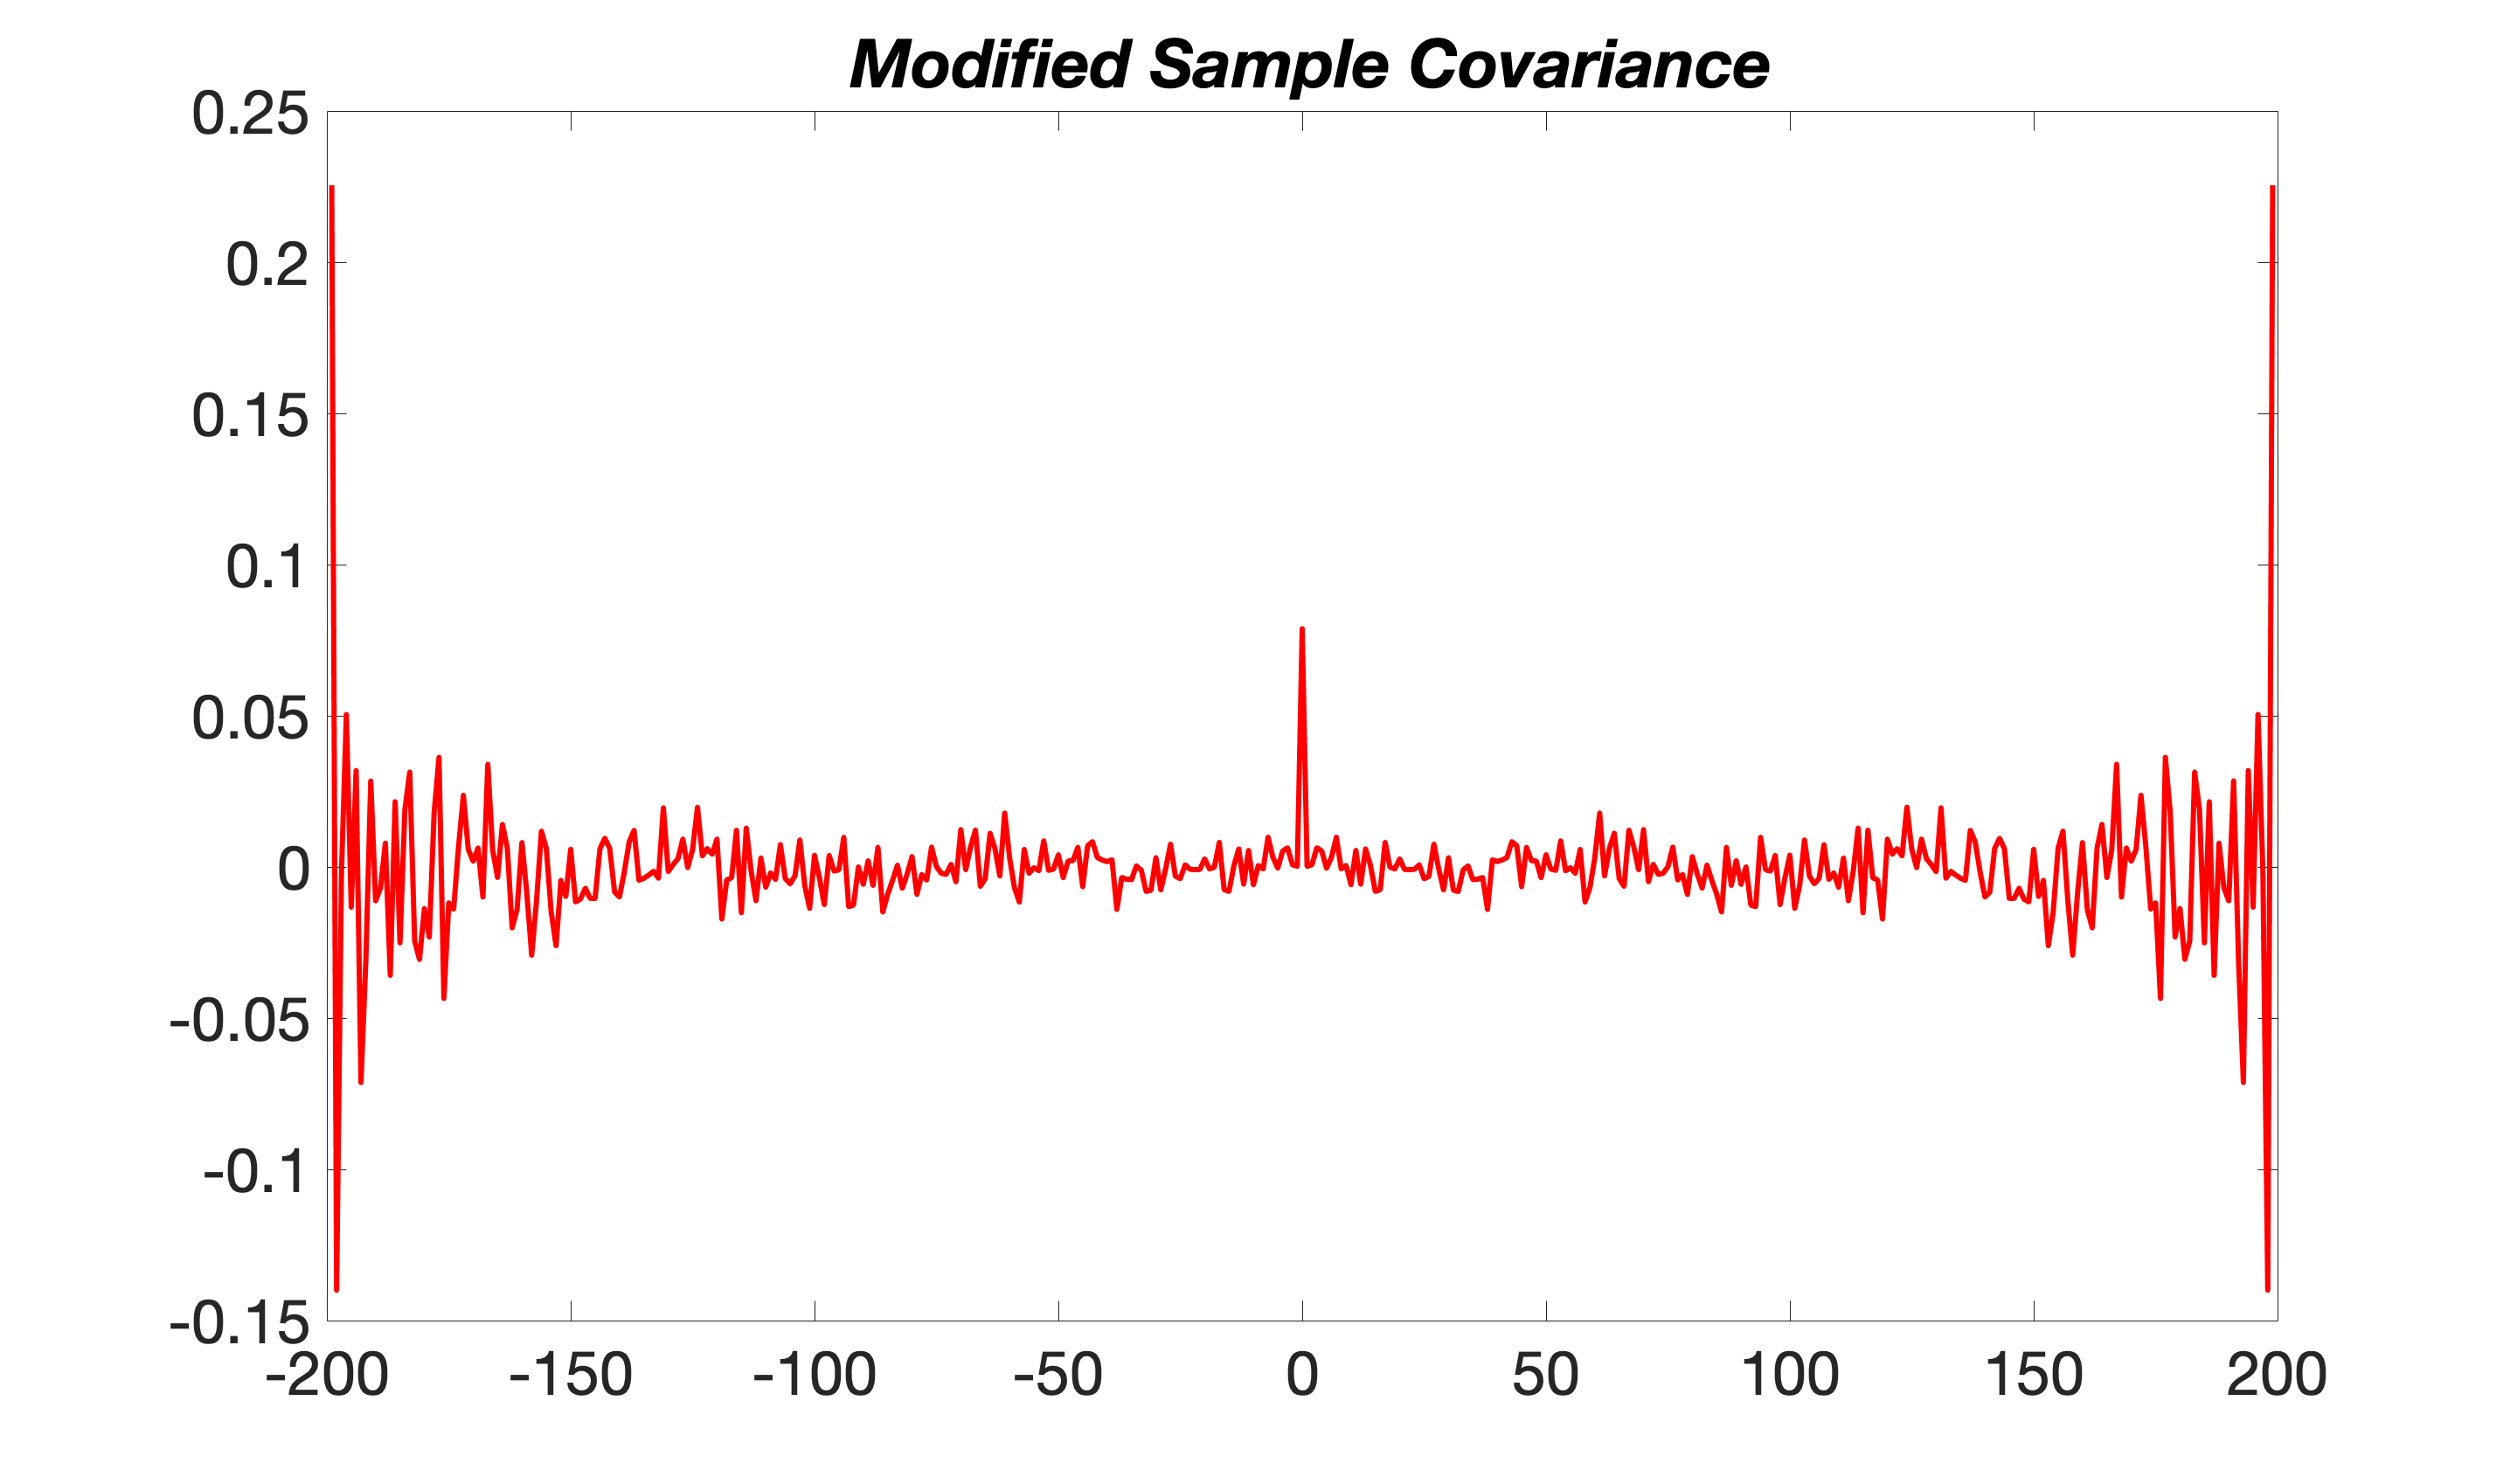
\includegraphics[width=8cm]{ass1_2.png}} }
    \qquad
    \subfloat[Unbiased Covariance]{ {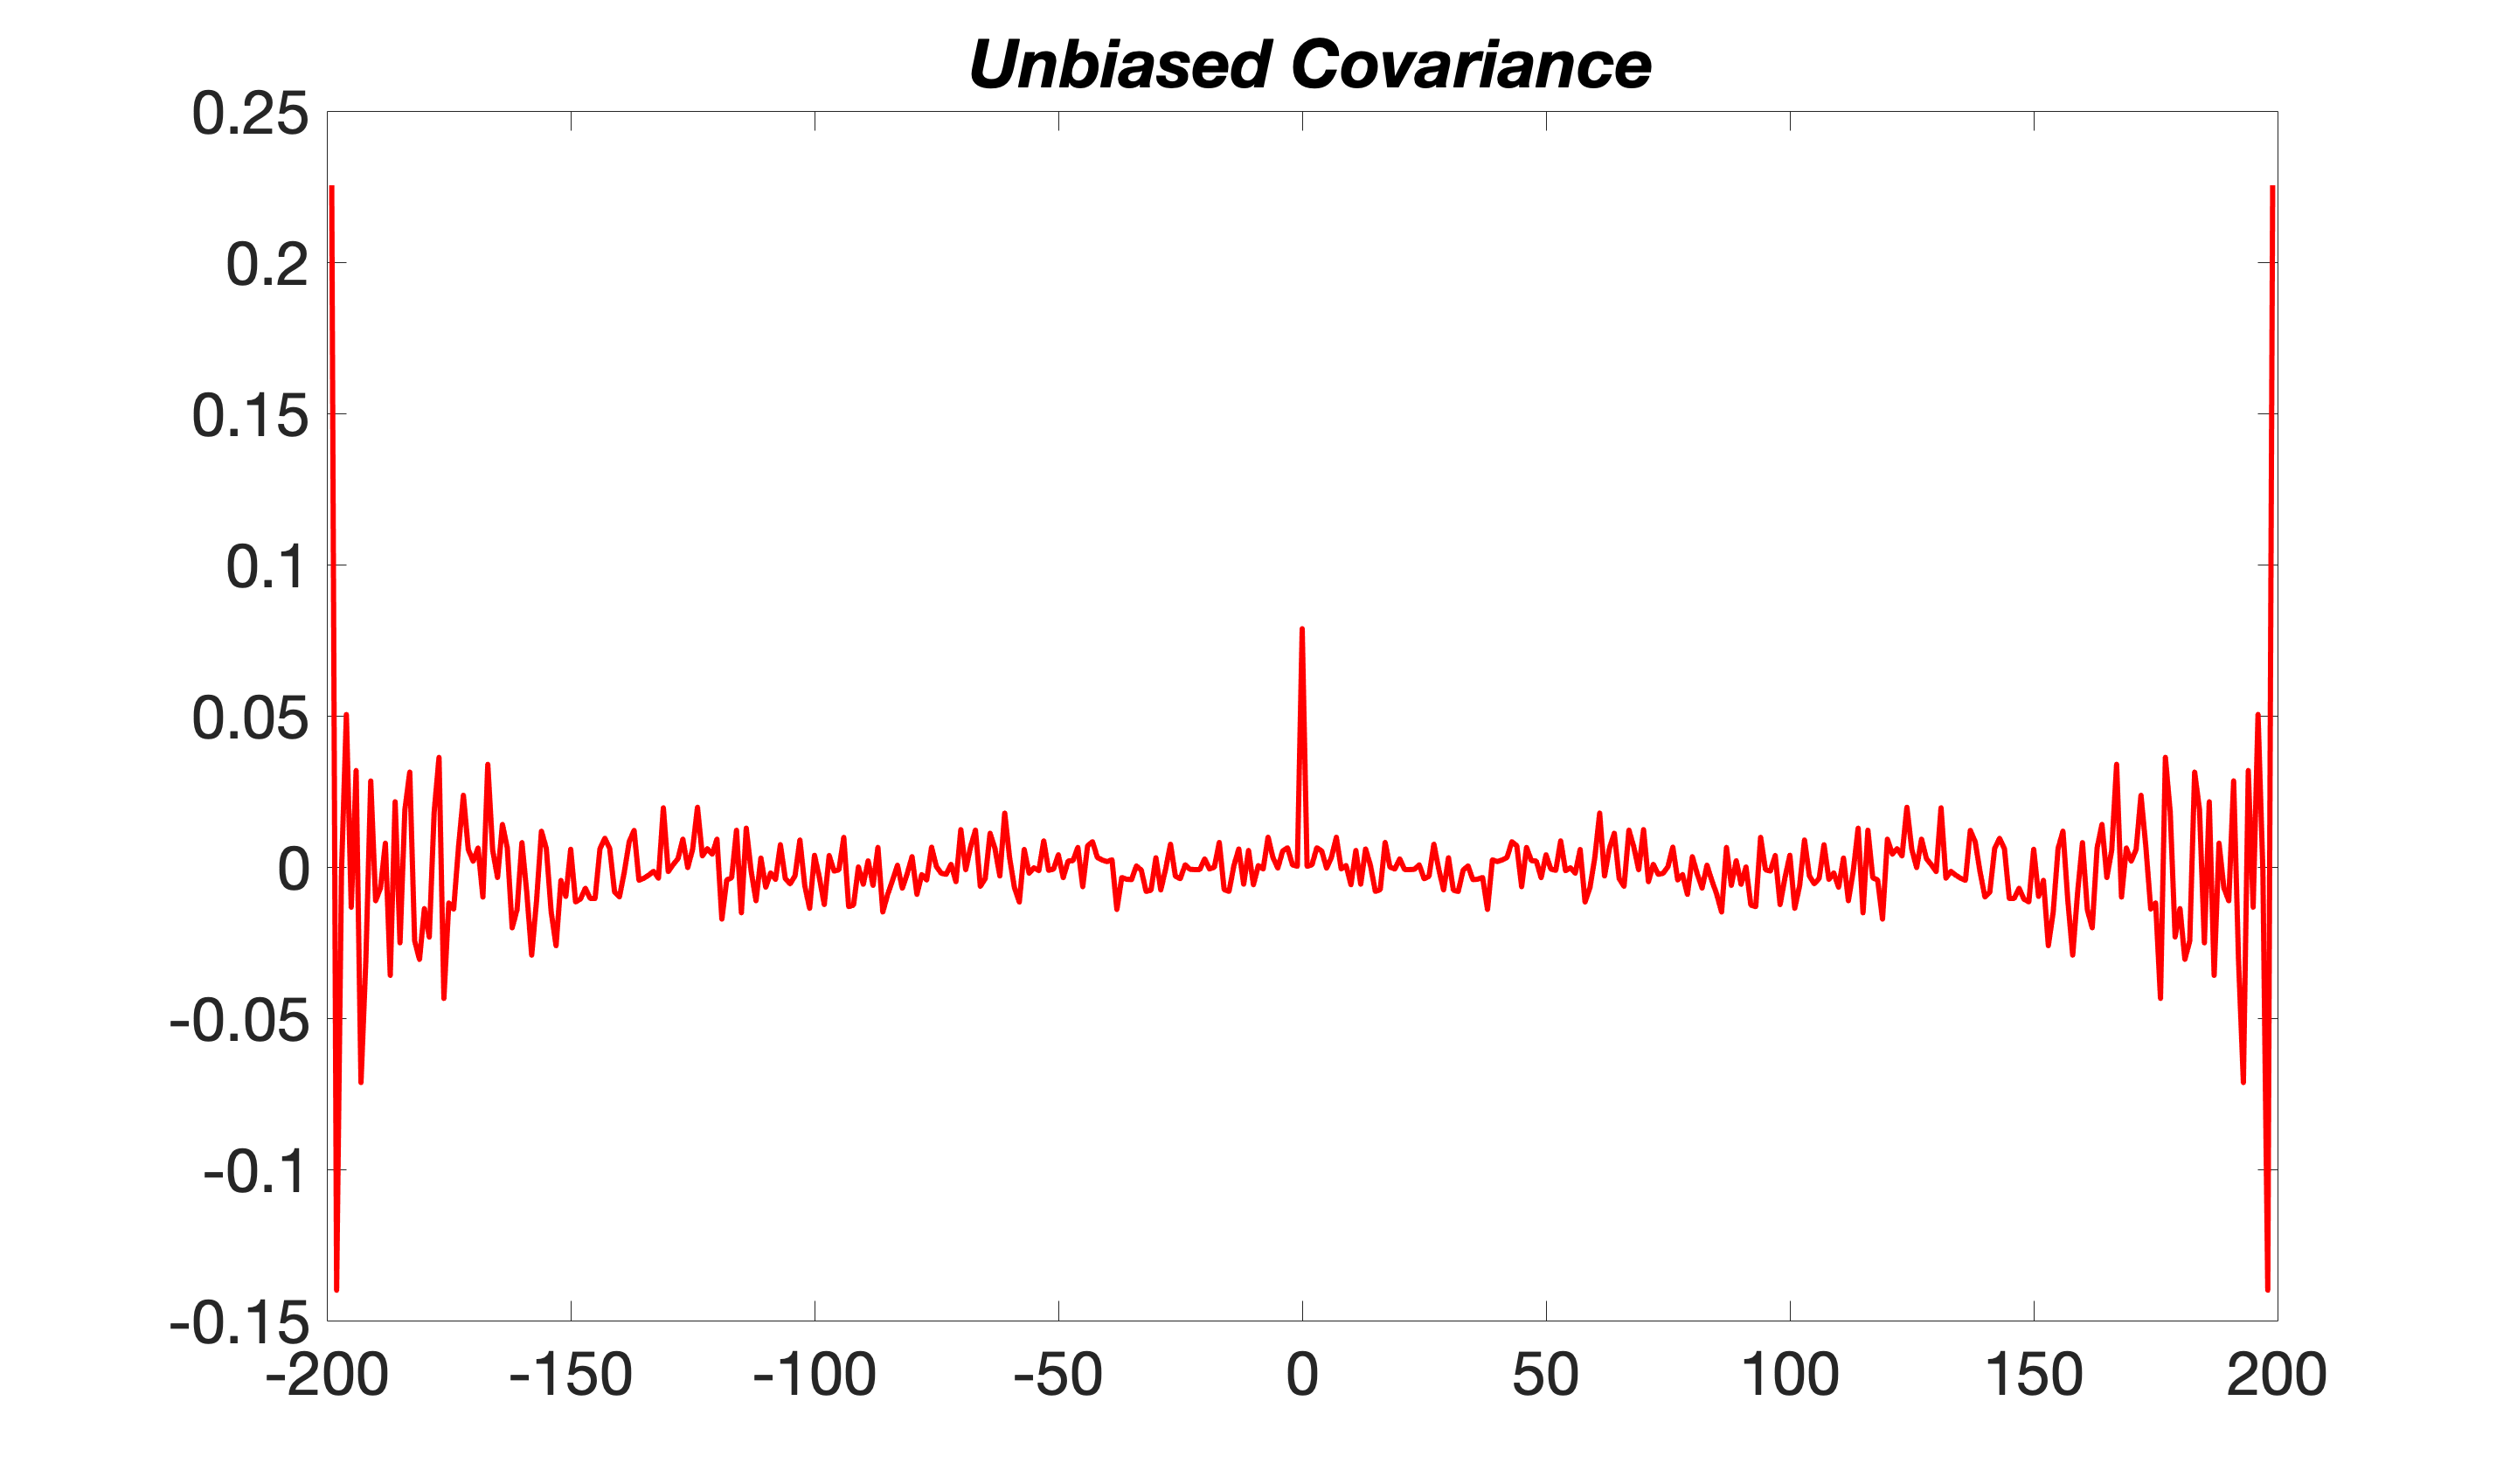
\includegraphics[width=8cm]{ass1_4.png} }}
    \caption{Covariances found using functions \texttt{covfct}(Modified Sample) and \texttt{xcov}(Unbiased)}
\end{figure}
\noindent If one covariance function is plot on x-axis and the other is plot on y-axis, it would be clear that they are equal which is shown in Figure 2.3. It can be concluded that all the outputs are symmetric.
\begin{figure}[H]
    \centering
   \subfloat[Uniform distribution]{ {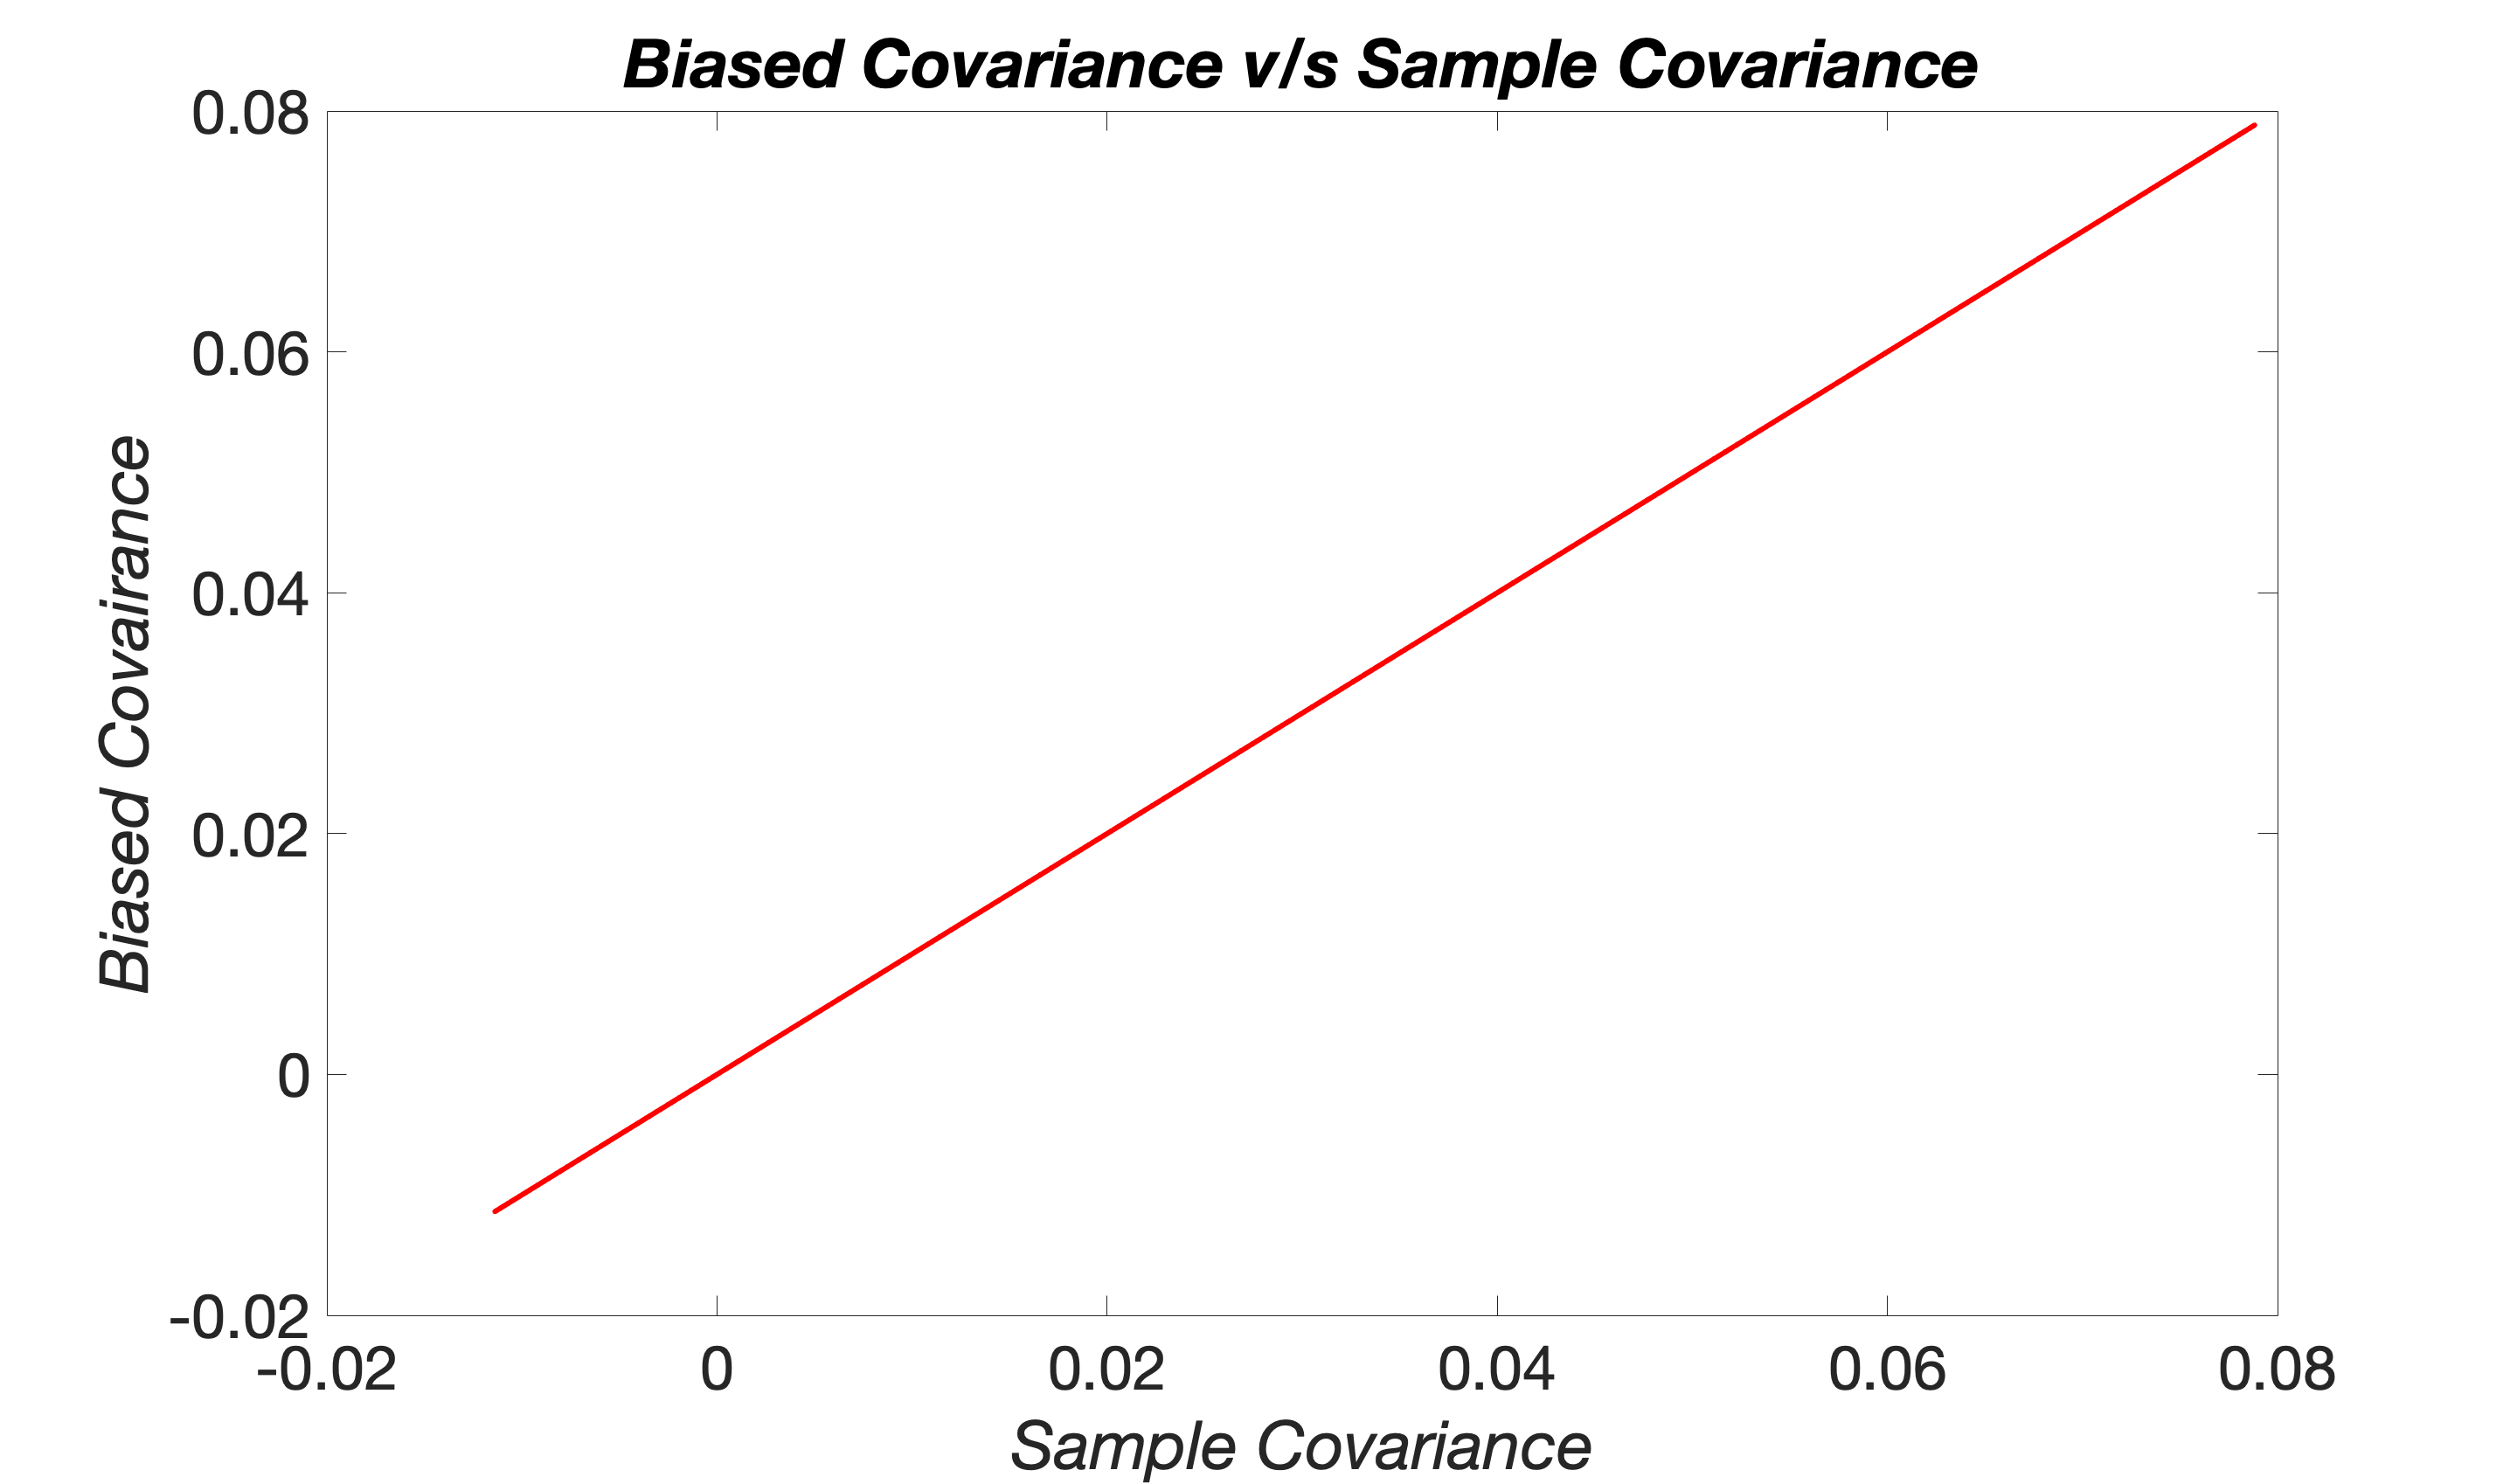
\includegraphics[width=8cm]{ass1_5.png}} }
    \qquad
    \subfloat[Standard normal distribution]{ {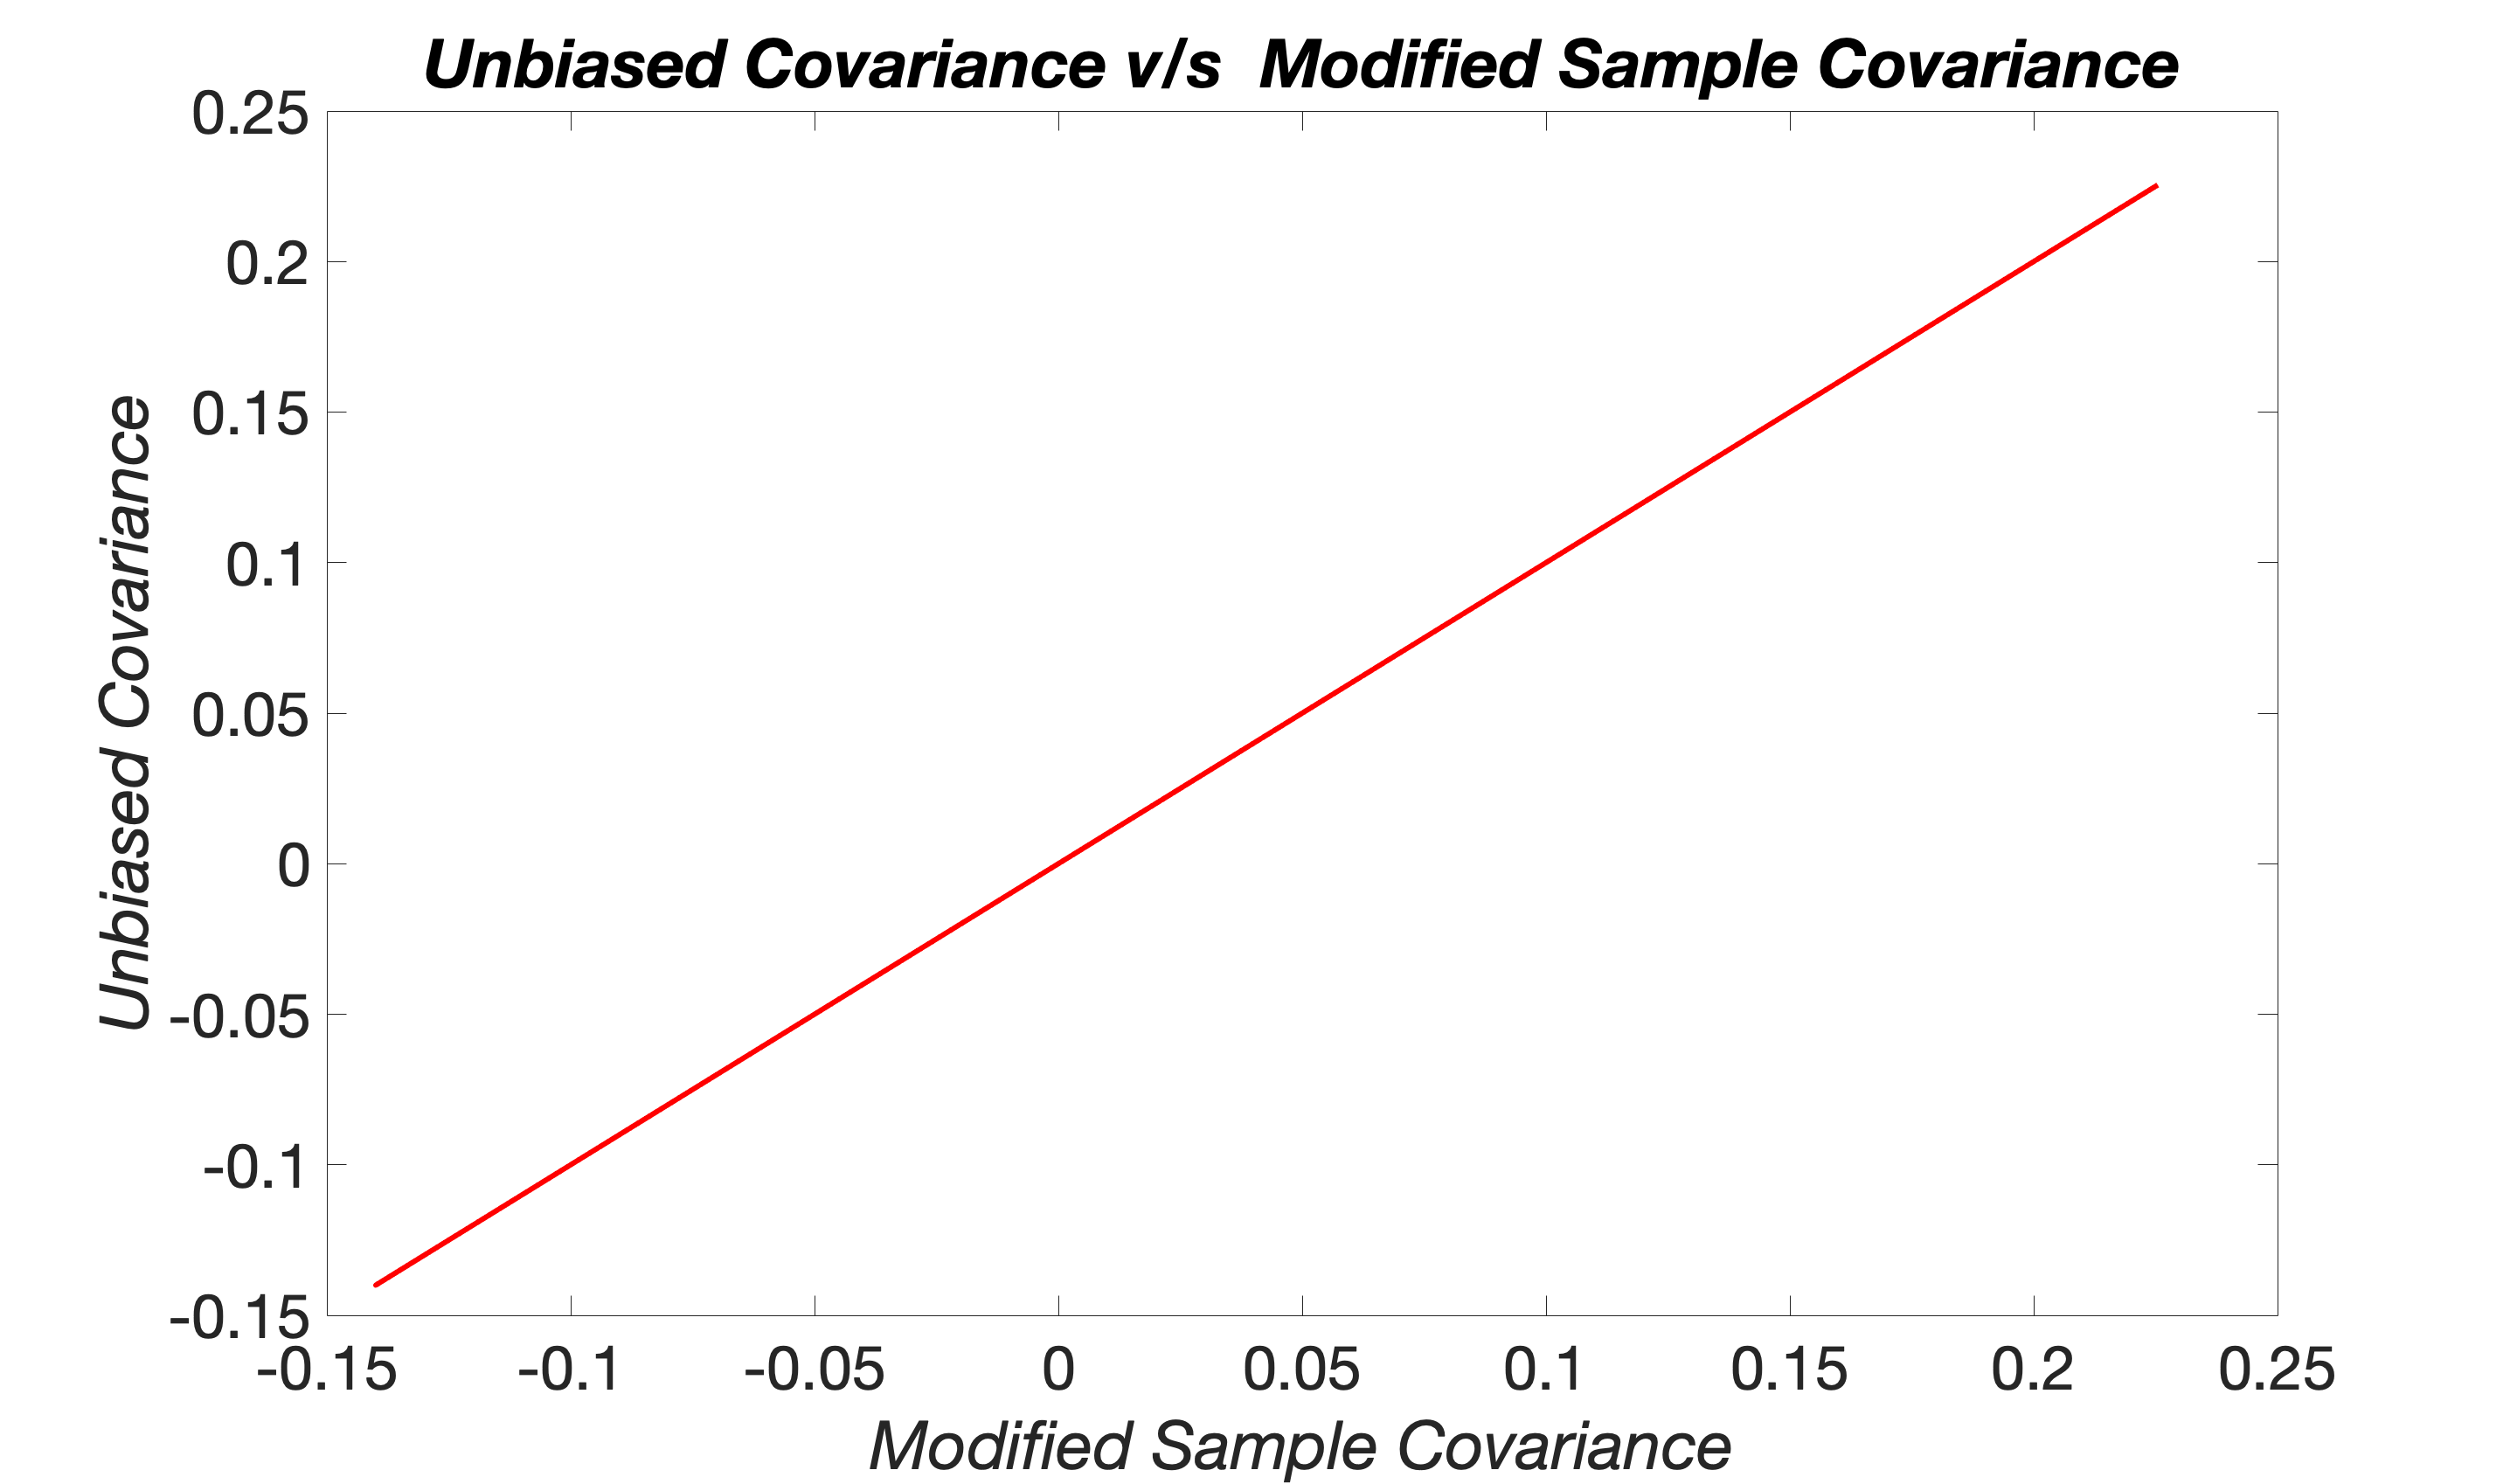
\includegraphics[width=8cm]{ass1_6.png} }}
   \caption{Comparison of the covariances}
   \end{figure}
\noindent \textbf{Inference:} The results obtained by the Matlab function \texttt{xcov biased} match the results of the sample covariance function, and the results of \texttt{xcov unbiased} match the results of the modified sample
covariance function. The sample covariance function is more accurate in case of a large number of observations because the variance converges to zero when the number of observations is getting very large. However, the modified sample variance function gives better results when the number of observations is limited.


%%%%%%%%%%% code 2 %%%%%
\section{ Generation of AR($p$) - processes} 
\noindent \textbf{Task:} Load \texttt{dat1\_2} that includes a realization of white noise. For the generation of an AR($p$) process you have to filter the white noise by a recursive filter with the filter coefficients $a_1 = 0.5, a_2 = 0.3, a_3 = 0.1, a_4 = 0.7, a_5 = 0.3.$ Use the MATLAB-function \texttt{filter}. Save the white noise and the AR ($\rho$) - process for later use in \texttt{dat4\_1}.
 \\

\noindent \textbf{Solution:}
\noindent The data which includes a realization of white noise is loaded at first. This white noise is filtered using the recursive filter with the filter coefficients $a_1 = 0.5, a_2 = 0.3, a_3 = 0.1, a_4 = 0.7, a_5 = 0.3.$We used the MATLAB function \texttt{filter} for this process and both white noise as well as AR($\rho$) - processes is saved in \texttt{dat4\_1}

\noindent \textbf{MATLAB code:}
\lstinputlisting{assignment4_2.m}

\noindent \textbf{Output:}
\noindent Figure 2.4 shows the impulse response of the filter.

\begin{figure}[H]
\centering
{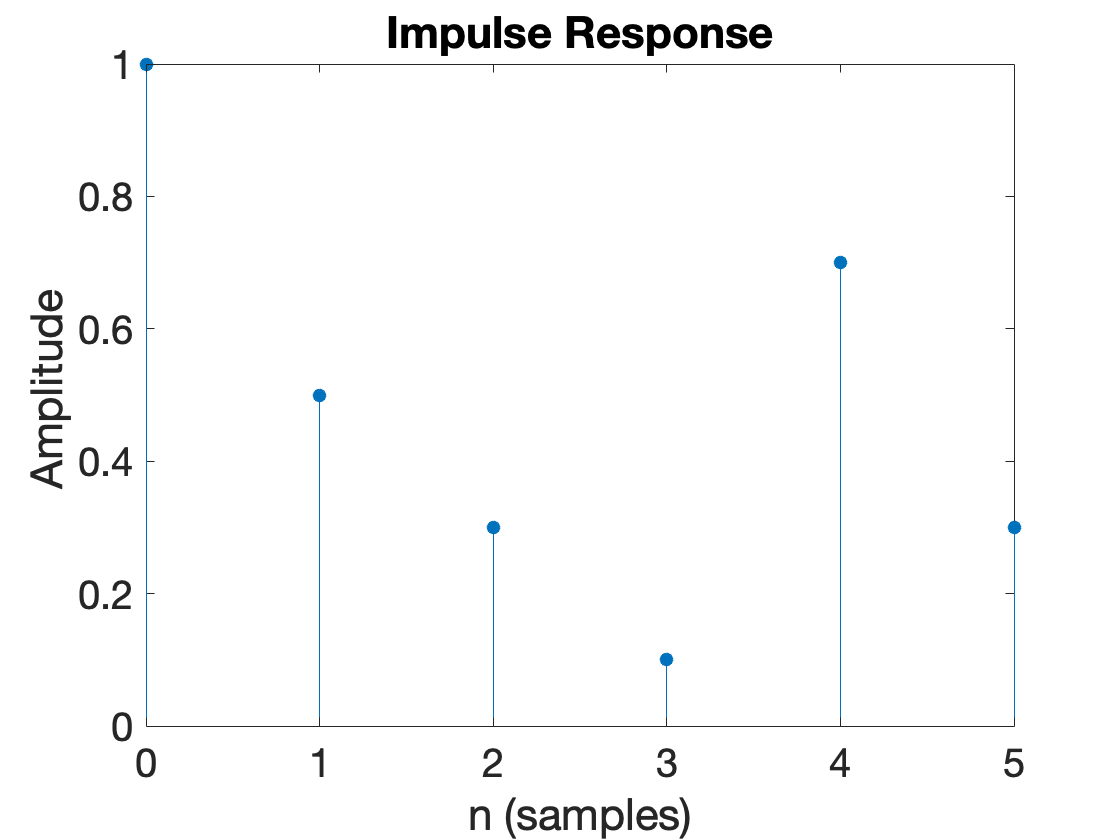
\includegraphics[scale=0.25]{ass2_1.png}}
\caption{Impulse response of the filter }
\end{figure}

\noindent \textbf{Inference:} The Auto-Regression process is been realized by the filtering the normally distributed random numbers using the Matlab function filter, with the given coefficients: a = [1,0.5,0.3,0.1,0.7,0.3], b = [1]. The mean value of the impulse response is zero.  After obtaining the coefficients the AR($p$)-process is being generated, and the data are saved for further processing.

%%%%%%%%%%%%%%% code 3 %%%%%
\newpage

\section{ LS-Estimation } \label{ LS-Estimation  }
\noindent \textbf{Task:} Carry out a LS - Estimation of the parameters $a_i(i=1,2,...,5)$ and the variance ${\sigma_Z}^2$of the AR($p$)-process.

\noindent \textbf{Solution:}  
\noindent The LS - Estimation of the parameters $a_i(i=1,2,...,5)$ and the variance ${\sigma_Z}^2$of the AR($p$)-process is carried out by the following code.

\noindent \textbf{MATLAB code:}
\lstinputlisting{assignment4_3.m}

\noindent \textbf{Output:}
\noindent The output after execution of the code is shown below. 
\begin{figure}[H]
\centering
{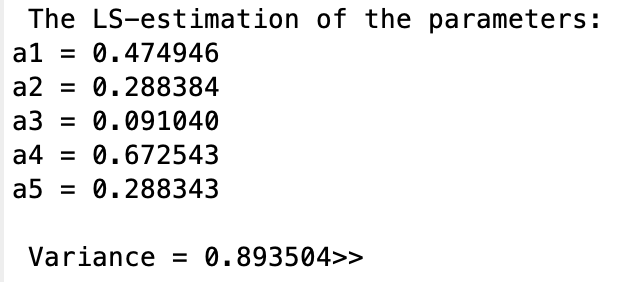
\includegraphics[scale=1.15]{ass3_1.png}}
\end{figure}

\noindent \textbf{Inference:} The parameters and the variance is calculated and shown above.

%%%%%%%% code 4 %%%%%


\section{ Estimating the order of a polynomial } \label{ Estimating the order of a polynomial}
\noindent \textbf{Task:} Estimate the order $p$ of the polynomial model. Therefore you have to depict the estimated variance versus the model order $p = 1,2,...,10.$ Consider the order that provides the smallest variance as the correct order. Estimate for that order the parameters $a_i$ for $i = 1,2,...,p.$

\noindent \textbf{Solution:} The same function \texttt{LSE} is used to obtain the variance of the polynomial model. The polynomial order $p$, is taken from 1 to 10 and the parameters at each order are shown in the output. 

\noindent \textbf{MATLAB code:}
\lstinputlisting{assignment4_4.m}
\noindent \textbf{Output:} The written code plots variance versus polynomial order. It can be seen that the  variance decreases drastically and after a point it remains constant. The plot can be seen in Figure 2.3.
\begin{figure}[H]
\centering
{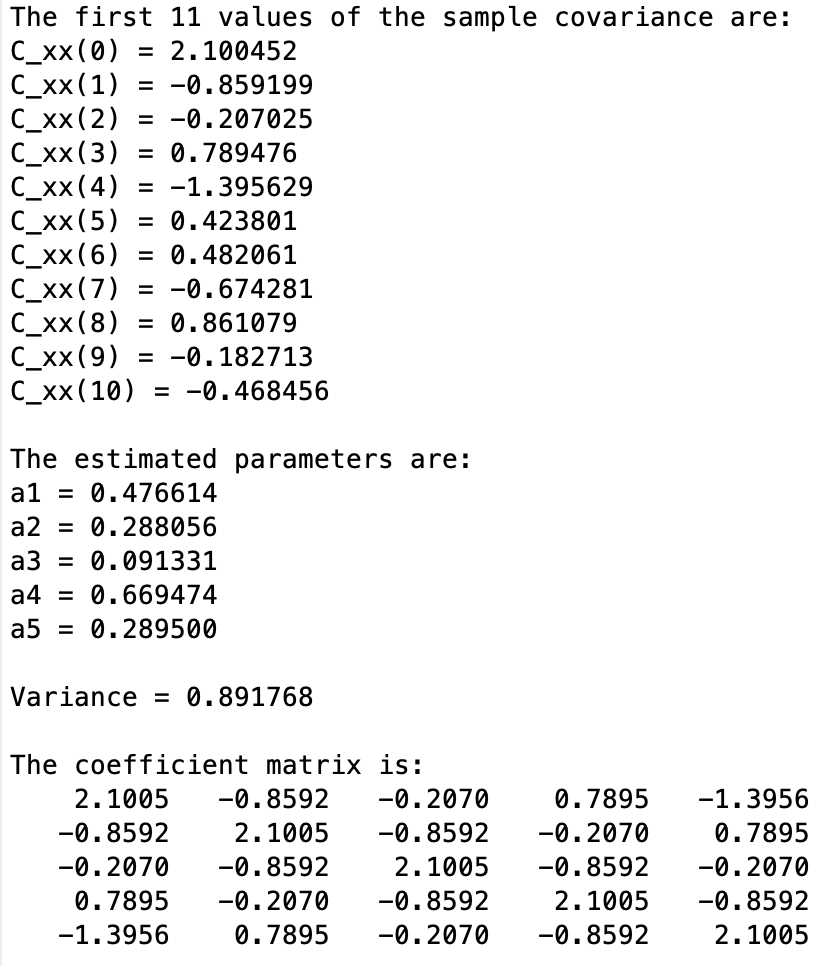
\includegraphics[scale=0.16]{ass4_1.png}}
\caption{Variance as a function of the polynomial order}
\label{Variance as a function of the polynomial order}
\end{figure}
\newpage
\noindent The output of the execution is shown below. The parameters for polynomial order 1 to 10 are printed and shown.

\noindent \textbf{Inference:} The variance reduces from 43.87 at $p = 1$ to 0.767 at $p = 3.$ Hence the polynomial of order 3 is considered to be the correct order. This is because, as the order increases further than 3, it remains almost constant. The parameters for the polynomial of order 3 are:  a = 4.77091, b = 2.47796, c = 1.187414 and d = -0.64021.
%%%%%%%%%%%  code 5  %%%%%

\section{Comparison of observations and estimated model}  \label{Comparison of observations and estimated model}
\noindent \textbf{Task:} For each of the models estimated above show the observations of the model ($x_i, y_i$) : $i = 1,2,...,N$ and the corresponding reconstructed model curve ($x_i, g(x_i)$) : $i = 1,2,...,N$ in one figure.
 
 \noindent \textbf{Solution:} We created a function \texttt{compare} inside the function \texttt{plotGraph} which used the values of the parameters from the previous exercise i.e., when $p = 3$ for polynomial model and $p = 1$ for the rest of the models to compare with the observed values from the data set which was previously created.\\
 
 \noindent \textbf{MATLAB code:}
\lstinputlisting{assignment4_5.m}

 \noindent \textbf{Output:}
 \noindent The output of the code is shown below. The estimated value is shown by a line while the observed value is represented by dots.
\begin{figure}[H]
\centering
{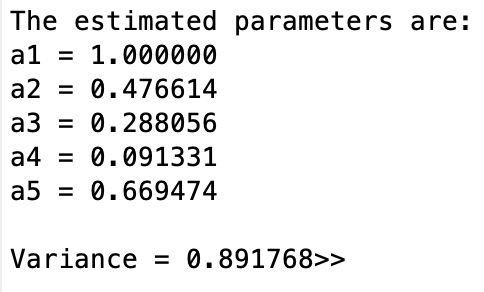
\includegraphics[scale=0.15]{ass5_1.png}}
\caption{LS-adjustment to a circle: estimating the centre }
\label{LS-adjustment to a circle: estimating the centre }
\end{figure}


\noindent \textbf{Inference:} We can infer that the observed value almost coincides with the estimated value. 

%%%%%% code 6 %%%%%%

\section{ LS-adjustment to a circle: estimating the centre  }  \label{ LS-adjustment to a circle: estimating the centre }
\noindent \textbf{Task:} Load \texttt{dat3\_2} containing a 100 $\times$ 2 matrix that represent the coordinates of 100 measurement points in the \textit{xy}-plane. Take a look at the measurement points and give from this the coordinates of the centre location. 


\noindent \textbf{Solution:} \texttt{dat3\_2} was loaded as mentioned in the task. It contains the matrix of data set $xy.$ We estimate and find the centre of the circle to be located at (4,2).\\ 

\noindent \textbf{MATLAB code:}
\lstinputlisting{assignment4_6.m}

\begin{figure}[H]
\centering
{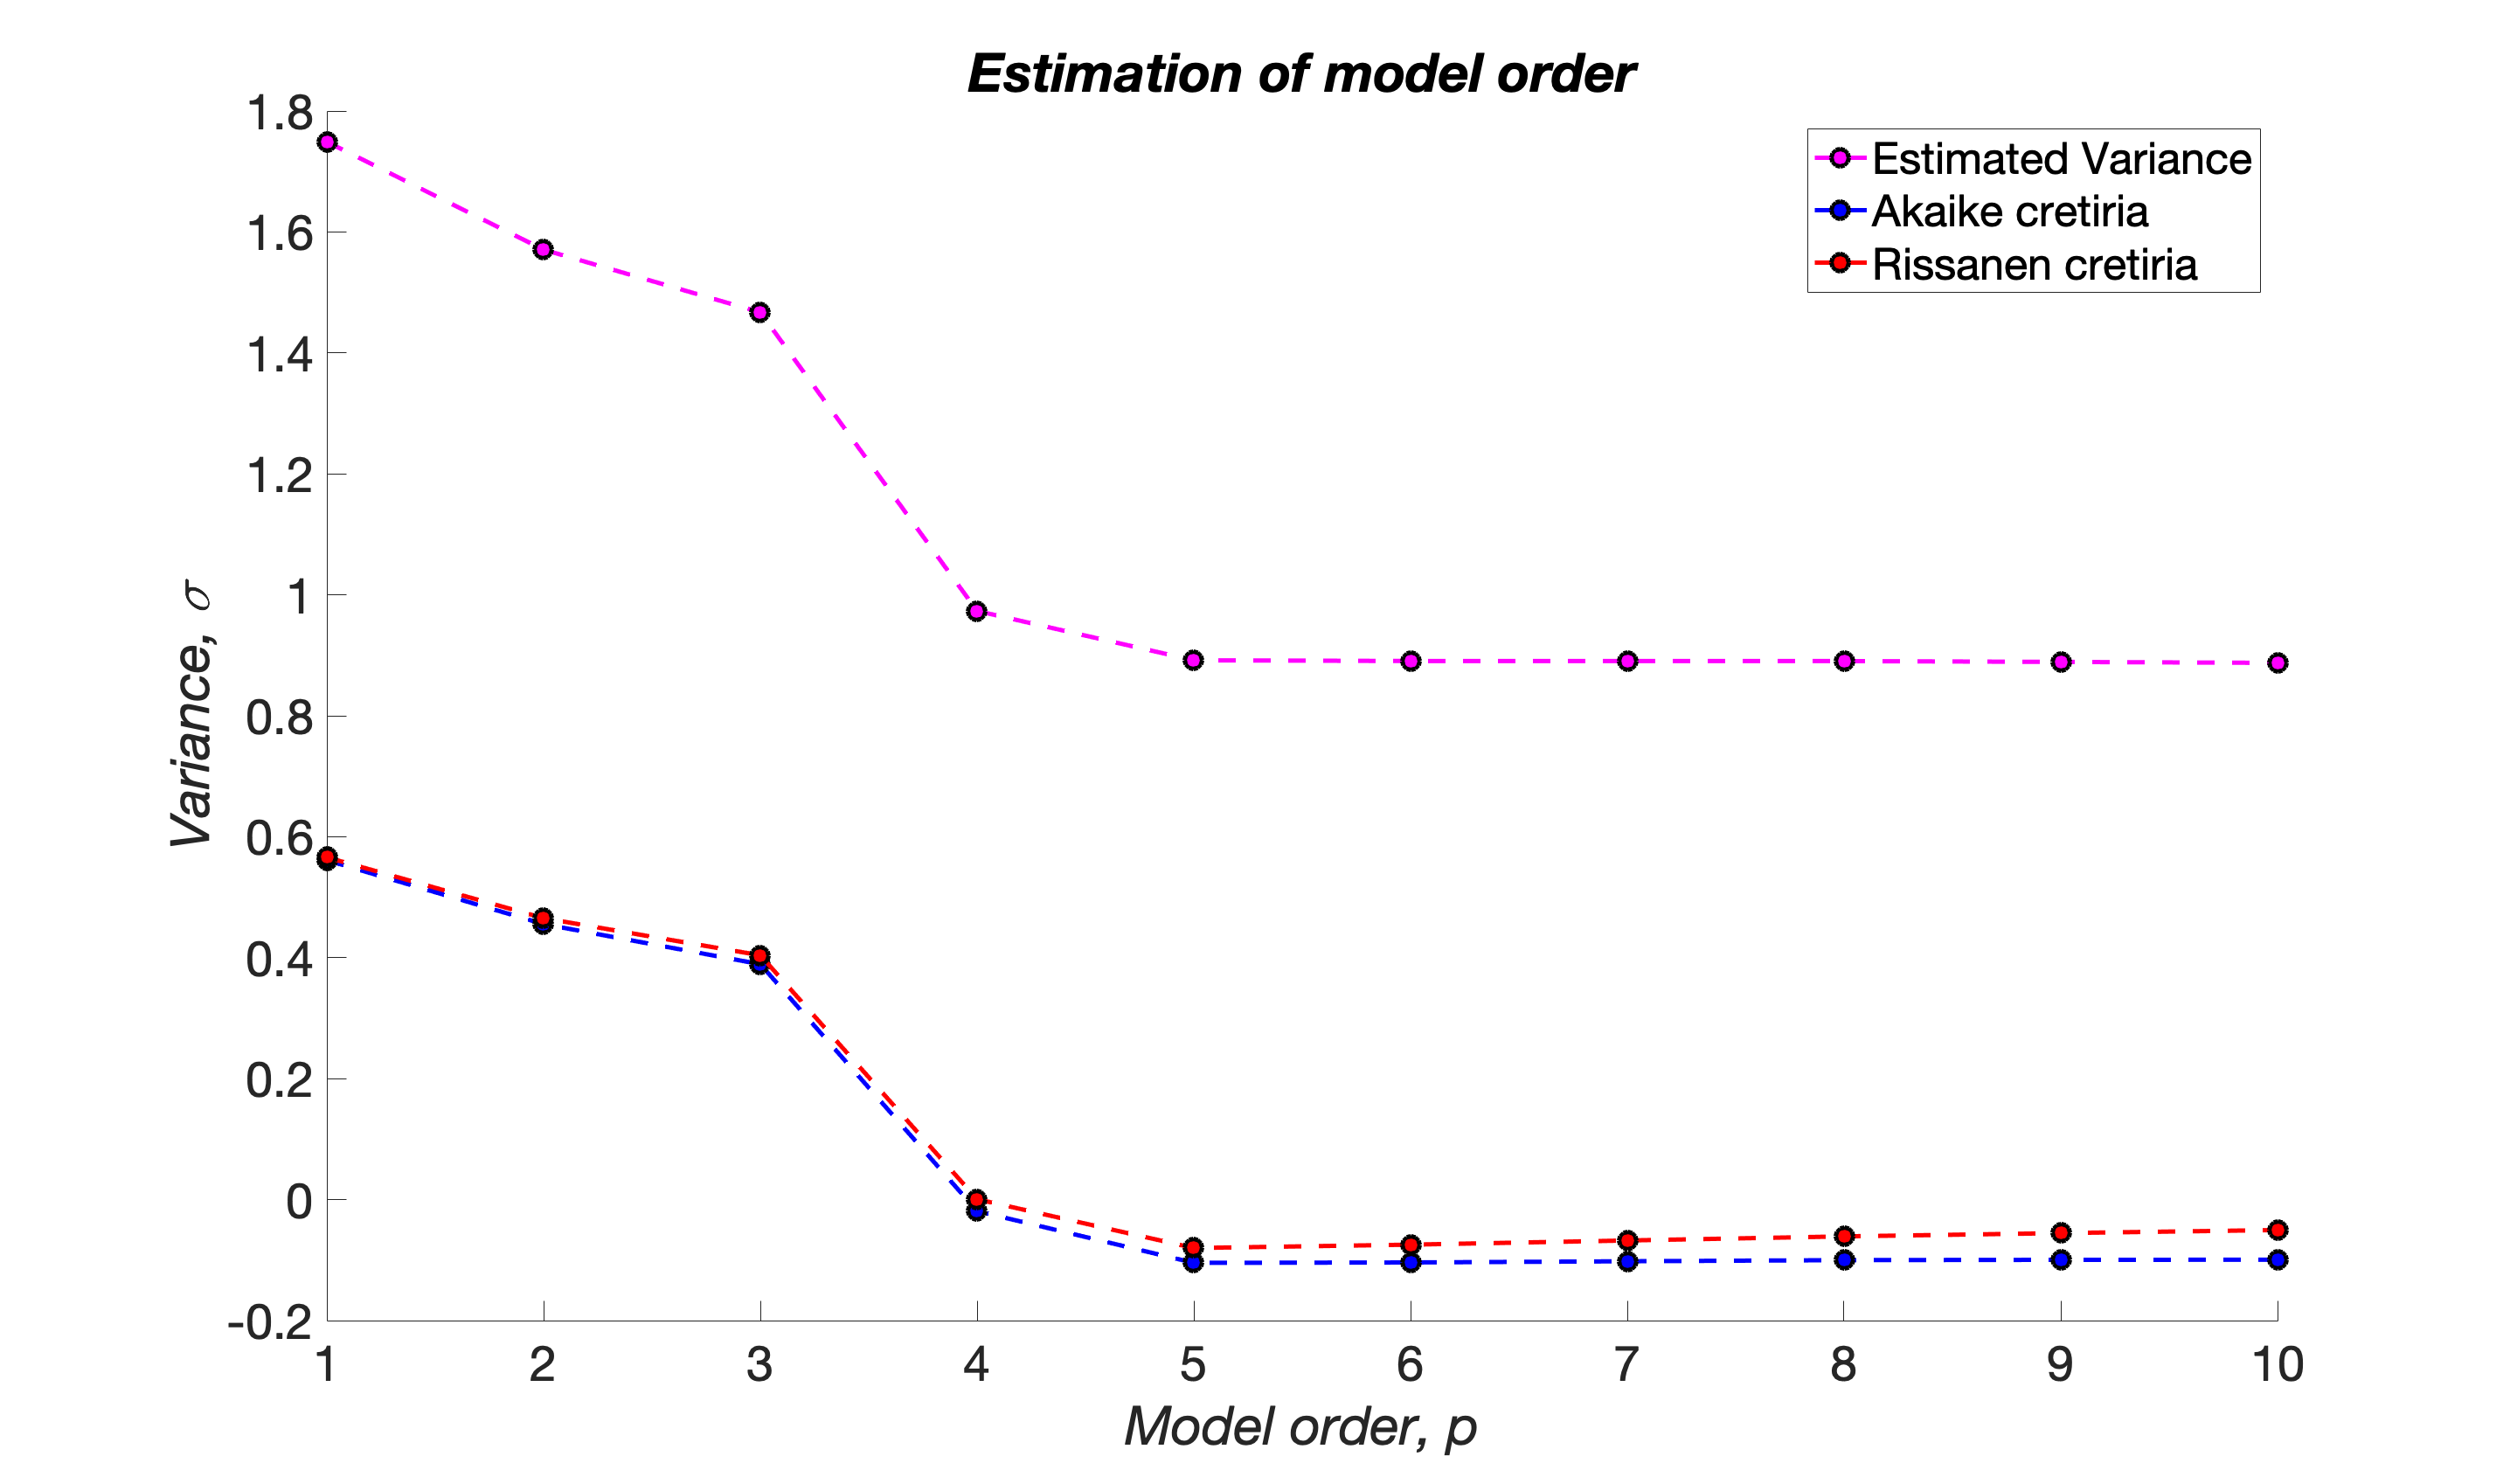
\includegraphics[scale=0.15]{ass6_1.png}}
\caption{LS-adjustment to a circle: estimating the centre }
\label{LS-adjustment to a circle: estimating the centre }
\end{figure}

\begin{figure}[H]
\centering
{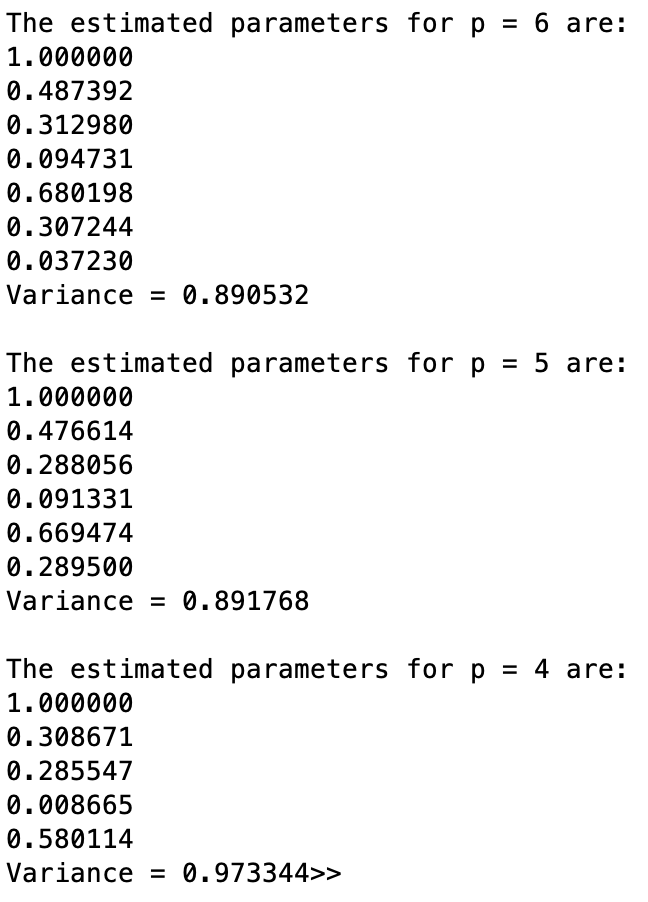
\includegraphics[scale=0.15]{ass6_2.png}}
\caption{LS-adjustment to a circle: estimating the centre }
\label{LS-adjustment to a circle: estimating the centre }
\end{figure}

\noindent \textbf{Inference:} The measurement points nearly takes the shape of a circle with centre at (4,2)


